\chapter{Confluence}

In this chapter, we prove a basic property of the lambda calculus,
called confluence.\index{confluence} Given a binary relation $\to$ on
a set $A$, an element $a \in A$ is confluent iff no matter which pair
of $\to$-paths we follow from $a$, ending in some elements $b$ and
$c$, there is a pair of $\to$-paths from $b$ and $c$ ending in a
common element $d$.  This can be expressed pictorially as:

\begin{center}
\begin{tikzpicture}
  \node at (0,2) (a){a};
  \node at (-2,0) (b){b};
  \node at (2,0) (c){c};
  \node at (0,-2) (d){d};

  \node at (.4,-1.85) {$*$};
  \node at (-.4,-1.85) {$*$};
  \node at (-1.85,.4) {$*$};
  \node at (1.85,.4) {$*$};

  \draw[->] (a) -- (b);
  \draw[->] (a) -- (c);
  \draw[->,dashed] (b) -- (d);
  \draw[->,dashed] (c) -- (d);  
\end{tikzpicture}
\end{center}

Confluence can be seen as a generalization of determinism
(Definition~\ref{def:det}), the property that whenever $a \to b$ and $a
\to c$, we have $b = c$.  For it might happen that we have paths from
$a$ that can reach distinct elements $b$ and $c$ (that is, $a \to^* b$
and $a \to^* c$, with $b \neq c$), but these elements can be joined
back at some element $d$ (so $b \to^*d$ and $c\to^*d$).  So $a$ is
nondeterministic, yet in a somewhat controlled way: no matter
which two paths we follow from $a$, there is always some way to
reconverge.

In this chapter, we will prove that the relation $\curva_\alpha \cup
\curva_\beta$ is confluent.  This relation subsumes the relation
$\betaa$ of single-step $\beta$-reduction with renaming
(Definition~\ref{def:betaa}), because it allows any sequence of
$\curva_\alpha$ and $\curva_\beta$ steps, while a non-trivial
$\betaa$-reduction sequence must end with a $\curva_\beta$ step.
Working with the more permissive relation will enable a cleaner
formulation of confluence.  The proof we will follow is attributed to
William Tait and Per Martin-L\"of (but never published by either of
them).  Some of our discussion is quite generic, however, and applies
to any binary relation $\to$ over some set of elements (not
necessarily terms).

We will use the notation $\abeta$ for the relation that we
will study in this chapter:

\begin{definition}
  \label{def:abeta}
  $\abeta$ is defined to be $\curva_\alpha \cup \curva_\beta$.
  \end{definition}

\section{The diamond property}

A property quite similar to confluence of a relation $\to$ is
the following:
\begin{definition}[Diamond property]
\label{def:diamond}
  An element $x$ has the diamond property with respect to relation
  $\to$ on set $A$ iff $x \to y$ and $x \to z$ imply that there exists an element $q$
  with $y \to q$ and $z \to q$. The relation $\to$ itself has the diamond
  property, denoted $\textit{Diamond}(\to)$, iff every element of $A$ has
  the diamond property with respect to $\to$.  \index{diamond property}
  \end{definition}
\noindent Pictorially, this is very similar to the diagram for confluence,
but without the stars:

\begin{center}
\begin{tikzpicture}
  \node at (0,1.75) (a){a};
  \node at (-1.75,0) (b){b};
  \node at (1.75,0) (c){c};
  \node at (0,-1.75) (d){d};


  \draw[->] (a) -- (b);
  \draw[->] (a) -- (c);
  \draw[->,dashed] (b) -- (d);
  \draw[->,dashed] (c) -- (d);  
\end{tikzpicture}
\end{center}

Indeed, an alternative definition of confluence of $\to$ is simply to say that $\to^*$ has the diamond property.
In this form, the following lemma states that reflexive-transitive closure preserves the diamond property:
\begin{theorem}[Star preserves diamond]
\label{thm:stardia}
  $\textit{Diamond}(\to)$ implies $\textit{Diamond}(\to^*)$
\end{theorem}
\begin{proof}
  Assume $\textit{Diamond}(\to)$ and $x$, $y$, $z$ with $x \to^*y$ and $x \to^* z$.  We proceed
  by induction on the derivation of $x \to^* y$ (recall the three rules defining the reflexive-transitive
  closure, in Figure~\ref{fig:rtcl}):

  \case{ }
  \[
  \infer{x \to^* y}{x \to y}
  \]
  \noindent Here we will proceed by an inner induction on the derivation of $x \to^* z$ to show that there
  is a $q$ with $y\to^*q$ and $z \to q$, for all $x$, $y$, and $z$ with $x\to y$.

  \case{ (inner)}
  \[
  \infer{x \to^* z}{x \to z}
  \]
  \noindent We have exactly the assumptions of the diamond property, so we can conclude that there is a $q$
  with $y \to q$ and $z \to q$.  Our inner induction requires us to show $y \to^* q$, which follows from
  this same inclusion rule whose inferences we are presently considering.

  \case{ (inner)}
  \[
  \infer{x \to^* x}{\ }
  \]
  \noindent We have learned in this case that $x = z$, since that is the only way the reflexivity
  rule could be applied to prove $x \to^*z$.  
  For whatever $q$ we select, we must prove $y \to^*q$ and $z \to q$.  
  Since $x = z$, it suffices to show $y \to^*q$ and $x \to q$.  Let us take $q$ to be $y$.
  So we must show $y \to^* y$, which follows by the reflexivity rule; and $x \to y$, which
  follows by assumption in this inner induction.

  \case{ (inner)}
  \[
  \infer{x \to^* z}{x \to^*w & w \to^* z}
  \]
  \noindent We may apply the induction hypothesis to the first premise of this
  inference.  So the $x$, $y$, and $z$ of the induction hypothesis are instantiated
  with $x$, $y$, and $w$, respectively.  The induction hypothesis then tells us that
  there is an element $q$ such that $y \to^*q$ and $w \to q$.  We may now apply the
  induction hypothesis to the second premise, where we
  instantiate $x$, $y$, and $z$ with $w$, $q$, and $z$, respectively.  This tells
  us that there is a $q'$ with $q\to^*q'$ and $z \to q'$.  Combining a couple of
  the facts we have so far (namely, $y\to^* q$ and $q\to^* q'$) using the
  transitivity rule gives us $y \to^* q'$.  And we have $z \to q'$.
  So we may take the element $q$ which we are supposed to identify, to be this $q'$.
  This concludes the inner induction.  Note that this induction could be (and often is)
  broken out as a separate lemma, since it does not need to invoke the outer induction
  hypothesis.
  
  We may now return to our outer induction:

  \case{ }
  \[
  \infer{x \to^* x}{\ }
  \]
  \noindent In this case, we have learned that $x = y$, since that is the only way a reflexivity
  inference could prove $x \to^* y$.  Our goal is to identify an element $q$ with $y \to^* q$ and $z \to^* q$,
  but since $x = y$, it suffices to find a $q$ with $x \to^* q$ and $z \to^* q$.  Take $q$ to be $z$, and
  we have $x \to^* z$ by assumption of this induction, and $z \to^* z$ by reflexivity.

  \case{ }
  \[
  \infer{x \to^* y}{x \to^* w & w \to^* y}
  \]
  \noindent By the induction hypothesis applied to the first premise, there is a $q$ with
  $w \to^* q$ and $z \to^* q$.  We may now apply the induction hypothesis to the second
  premise, instantiating $x$, $y$, and $z$ with $w$, $y$, and $q$, respectively.  This
  produces a $q'$ with $y\to^* q'$ and $q\to^* q'$.  Let us take $q'$ to be the $q$ required
  by the theorem.  Since $z\to^*q$ and $q\to^* q'$, we have $z \to^* q'$ by transitivity;
  and $y\to^* q'$ was already concluded.
  

  \end{proof}

Thanks to Theorem~\ref{thm:stardia}, we know that if we would like to establish confluence of $\abeta$, it
would suffice to prove that this relation has the diamond property.  But this is easily seen
not to be the case.  Consider the diagram in Figure~\ref{fig:betanodia}.  The term at the peak (top) of the diagram
has two redexes, shown underlined.  Down the left side of the peak we reduce the leftmost redex, and down the right
side, the rightmost.  We can indeed join the resulting terms, at term $z\ z$, but this requires two steps along the
left side of the valley (running diagonally right to $z\ z$), while needing just one step along the right
side of the valley.  This example shows:

\begin{theorem}
  $\abeta$ lacks the diamond property
\end{theorem}

It is the beautiful observation at the heart of the Tait--Martin-L\"of proof of confluence that
while $\beta$-reduction lacks the diamond property, still another relation $\Pred^\alpha$ can be defined which
satisfies the diamond property, and where $(\Pred^\alpha)^* = \betaa^*$.  This will lead us to our goal,
thanks to the following theorem:
\begin{theorem}
  \label{thm:tml}
  Let $S$ be a relation on a set $A$, and suppose that there is a relation $R$ on $A$ such that
  $\textit{Diamond}(R)$ and $R^* = S^*$.  Then $S$ is confluent.
\end{theorem}

\begin{proof}
  Confluence
  of $S$, is equivalent to $\textit{Diamond}(S^*)$.  Since $R^* = S^*$ by assumption, it suffices
  then to prove $\textit{Diamond}(R^*)$.  By Theorem~\ref{thm:stardia}, this follows
  from $\textit{Diamond}(R)$, which we have by assumption.
\end{proof}

Actually, the task of confluence is made even easier by observing the following:
\begin{lemma}
  If $S \subseteq R \subseteq S^*$, then $R^* = S^*$.
\end{lemma}
\begin{proof}
  By monotonicity of the reflexive-transitive closure operator (Lemma~\ref{lem:starmono}),
  $S \subseteq R$ implies $S^* \subseteq R^*$.  So we have inclusions both directions
  between $S^*$ and $R^*$, implying (in set theory) that they are equal.
  \end{proof}

\noindent So to use Theorem~\ref{thm:tml}, by this lemma, we just need to identify some relation
intermediate between $\abeta$ and $\abeta^*$, which satisfies the diamond property.  This relation
is $\Pred^\alpha$, defined next.

\begin{figure}

  \begin{center}
    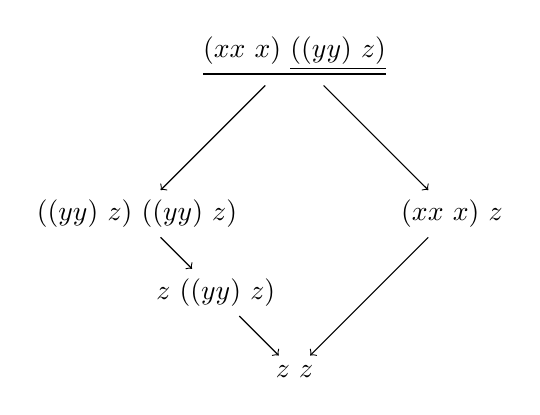
\begin{tikzpicture}
      \node at (0,2)(a){$\underline{(\lam{x}{x\ x})\ \underline{((\lam{y}{y})\ z)}}$};
      \node at (-2,0)(b){$((\lam{y}{y})\ z)\ ((\lam{y}{y})\ z)$};
      \node at (-1,-1)(c){$z\ ((\lam{y}{y})\ z)$};
      \node at (2,0)(d){$(\lam{x}{x\ x})\ z$};
      \node at (0,-2)(e){$z\ z$};

      \draw[->] (a) -- (b);
      \draw[->] (b) -- (c);
      \draw[->] (c) -- (e);
      \draw[->] (a) -- (d);
      \draw[->] (d) -- (e);
      \end{tikzpicture}
    \end{center}

\caption{Counterexample showing that $\beta$-reduction lacks the diamond property.}
\label{fig:betanodia}

\end{figure}

\section{Parallel reduction}

In this section, we define a relation $\Pred^\alpha$ for parallel reduction with renaming\index{parallel reduction}\index{$\Pred^\alpha$}.  This relation will be the desired
intermediate relation between $\abeta$ and $\abeta^*$, with the diamond property.  $\Pred$ is defined
by the rules of Figure~\ref{fig:pred} (i.e., $\Pred$ is the set of pairs $(t,t')$ such that $t\ \Pred\ t'$ has a finite
derivation using those rules).  It allows reduction, in a single step, of any subset of the redexes of the first related term,
to obtain the second.  One could reduce a single redex, several redexes (even nested ones), or no redexes at all.

We then define $\Pred^\alpha$ from $\Pred$ similarly to the way we defined $\betaa$ from
$\betaa_\beta$ (Definition~\ref{def:betaa})\index{$\Pred$}:

\begin{definition}
  $\Pred^\alpha$ is $=_\alpha\Pred $.
\end{definition}
\noindent So one takes an $\alpha$-equivalence step, then a $\Pred$ step.

\newcommand{\predvar}[0]{\infer{x \Pred x}{\ }}

\newcommand{\predlam}[0]{\infer{\lam{x}{t} \Pred \lam{x}{t'}}{t \Pred t'}}

\newcommand{\predapp}[0]{\infer{t_1\ t_2 \Pred t_1'\ t_2'}{t_1 \Pred t_1' & t_2 \Pred t_2'}}

\newcommand{\predbeta}[0]{\infer{(\lam{x}{t_1})\ t_2 \Pred [t_2'/x]t_1'}{t_1 \Pred t_1' & t_2 \Pred t_2'}}

\begin{figure}
\[
\begin{array}{lllllll}
\predvar

& \ &

\predlam

& \ &

\predapp

& \ &

\predbeta
 
\end{array}
\]
\caption{The definition of parallel reduction}
\label{fig:pred}
\end{figure}

Intuitively, we can see that $\Pred$ is intermediate between $\curva_\beta$ and $\curva_\beta^*$, because
it allows reducing any subset of the term's redexes.  Critically, though, it does not allow reduction
of \emph{created redexes}.\index{$\beta$-redex!created}  These are redexes that appear when a variable is replaced by a $\lambda$-abstraction.  For example, we have the reduction
\[
(\lam{x}{x\ y})\ \lam{z}{z}\ \curva_\beta (\lam{z}{z})\ y
\]
\noindent The latter term is a created redex, because there is no corresponding redex in the starting term, from which it is derived.

\subsection{Examples}

Here are some examples of parallel reduction.

\begin{enumerate}
\item Here are all the terms to which $(\lam{x}{x\ x})\ ((\lam{y}{y})\ z)$ parallel reduces:
  \begin{enumerate}
  \item $(\lam{x}{x\ x})\ ((\lam{y}{y})\ z)$, which is the starting term itself;
  \item $(\lam{x}{x\ x})\ z$, where the right redex in the starting term has been contracted;
  \item $((\lam{y}{y})\ z)\ ((\lam{y}{y})\ z)$, where the left redex has been contracted; and
  \item $z\ z$, where both redexes have been contracted.
  \end{enumerate}

  The derivation of the parallel reduction to the last of these is (for an example):

  \[
  \infer{(\lam{x}{x\ x})\ ((\lam{y}{y})\ z) \Pred z\ z}
        {\infer{x\ x \Pred x\ x}{\infer{x \Pred x}{\ } & \infer{x \Pred x}{\ }} & 
          \infer{(\lam{y}{y})\ z \Pred z}
                {\infer{y \Pred y}{\ } &
                  \infer{z \Pred z}{\ }}}
   \]

 \item We have the following parallel reduction:
   \[
   (\lam{x}{\lam{y}{x\ y}})\ (\lam{x}{\lam{y}{x\ y}}) \Pred \lam{y}{(\lam{x}{\lam{y}{x\ y}})\ y}
   \]
   \noindent This same starting term requires $\alpha$-equivalence to reduce further:
   \[
   \begin{array}{ll}
     \underline{(\lam{x}{\lam{y}{x\ y}})\ (\lam{x}{\lam{y}{x\ y}})} &\curva_\beta \\
     \lam{y}{(\lam{x}{\underline{\lam{y}{x\ y}}})\ y} & \curva_a \\
     \lam{y}{\underline{(\lam{x}{\lam{w}{x\ w}})\ y}} & \curva_\beta \\
     \lam{y}{\lam{w}{y\ w}} & \
   \end{array}
   \]
   \noindent But with parallel reduction, as long as all bound variables are distinct from the free variables,
   $\alpha$-equivalence is not required for a single $\Pred$-step.  And a single $\Pred$-step cannot reduce the starting term of this example past where the next redex is created.

\end{enumerate}

\subsection{Basic properties of parallel reduction}

\begin{lemma}
  \label{lem:predrefl}
  $t \Pred t$ for all terms $t$.
\end{lemma}
\begin{proof}
  The proof is by induction on $t$.

  \case{ } $t$ is a variable $x$. Then we may construct this derivation:
  \[
  \infer{x \Pred x}{\ }
  \]
  
\case{ } $t$ is an application $t_1\ t_2$ for some $t_1$ and $t_2$. Then we may construct:
\[
\infer{t_1\ t_2 \Pred t_1\ t_2}{\infer[\textit{IH}]{t_1 \Pred t_1}{\ } & \infer[\textit{IH}]{t_2 \Pred t_2}{\ }}
\]

\case{ } $t$ is a $\lambda$-abstraction $\lam{x}{t'}$ for some $x$ and $t'$. Then we construct:
\[
\infer{\lam{x}{t'} \Pred \lam{x}{t'}}{\infer[\textit{IH}]{t' \Pred t'}{\ }}
\]
\end{proof}

\begin{lemma}
  \label{lem:betapar}
  $\abeta\ \subseteq\ \Pred^\alpha$.
\end{lemma}
\begin{proof}
  It suffices to assume $t \abeta t'$ for some $t$ and $t'$,
  and show $t \Pred^\alpha t'$.  Since $\abeta$ is defined (Definition~\ref{def:abeta}) to be $\curva_\alpha \cup \curva_\beta$,
  let us consider each possibility.  If we have $t \curva_\alpha t'$, then we have $t \Pred^\alpha t'$, because 
  \begin{enumerate}
  \item $t =_\alpha t'$, and
  \item $t' \Pred t'$, by Lemma~\ref{lem:predrefl}
  \end{enumerate}
  \noindent So we get $t =_\alpha t' \Pred t'$, which suffice to prove $t \Pred^\alpha t'$ (by definition of relational composition).

  Now suppose we have $t \curva_\beta t'$.  Then the proof is by
  induction on the derivation of $t \curva_\beta t'$ (via the rules of
  Figure~\ref{fig:betar}).

  \case{ }
  \[
  \infer{(\lam{x}{t})\ t'\ \curva_\beta\ [t'/x]t}{\ }
  \]
  \noindent We may construct the following, where we invoke Lemma~\ref{lem:predrefl} where indicated, so that we can limit
  the $\beta$-reduction rule for $\Pred$ just to this redex $(\lam{x}{t})\ t'$:
  \[
  \infer{(\lam{x}{t})\ t' \Pred [t'/x]t}
        {\infer[\textit{\ref{lem:predrefl}}]{t \Pred t}{\ } & \infer[\textit{\ref{lem:predrefl}}]{t' \Pred t'}{\ }}
  \]
        

  \case{ }
  \[
  \infer{\lam{x}{t}\ \curva_\beta\ \lam{x}{t'}}{t\ \curva_\beta\ t'}
  \]
  \noindent We construct:
  \[
  \infer{\lam{x}{t} \Pred \lam{x}{t'}}{\infer[\textit{IH}]{t \Pred t'}{t\ \curva_\beta\ t'}}
  \]

  \case{ }
  \[
  \infer{t_1\ t_2\ \curva_\beta\ t_1'\ t_2}{t_1\ \curva_\beta\ t_1'}
  \]
  \noindent Construct the following, again invoking Lemma~\ref{lem:predrefl}:
  \[
  \infer{t_1\ t_2\ \Pred\ t_1'\ t_2}{\infer[\textit{IH}]{t_1 \Pred t_1'}{t_1\ \curva_\beta\ t_1'} &
                                    \infer[\textit{\ref{lem:predrefl}}]{t_2 \Pred t_2}{\ }}
  \]

  \case{ }
  \[
  \infer{t_1\ t_2\ \curva_\beta\ t_1\ t_2'}{t_2\ \curva_\beta\ t_2'}
  \]
  \noindent Similarly to the previous case, construct:
  \[
  \infer{t_1\ t_2\ \Pred\ t_1\ t_2'}{\infer[\textit{\ref{lem:predrefl}}]{t_1 \Pred t_1}{\ }&
                                    \infer[\textit{IH}]{t_2 \Pred t_2'}{t_2\ \curva_\beta\ t_2'} }
  \]
  
        
  \end{proof}

\begin{lemma}
  \label{lem:predmbeta}
  $\Pred^\alpha\ \subseteq\ \abeta^*$
\end{lemma}
\begin{proof}
  Assume $t \Pred^\alpha t'$.  This implies that there exists some $t''$ with
  \[
  t =_\alpha t'' \Pred t'
  \]
  \noindent Since $\abeta$ includes $\curva_\alpha$ by definition, we have
  $t \abeta^* t''$.  So it suffices to show $t'' \abeta^* t'$.  In fact,
  we will show the stronger property $t'' \curva_\beta^* t'$.  This
  is done by  induction on the assumed
  derivation of $t'' \Pred t'$.

  \case{ }
  \[
  \predvar
  \]
  \noindent We construct:
  \[
  \infer{x \betaa_\beta^* x}{\ }
  \]

  \case{ }
  \[
  \predlam
  \]
  \noindent We construct the following, making use of
  Lemma~\ref{lem:comprtc} which implies that the compatible closure of $(\betaa_\beta^*)$
  is the same as just $\betaa_\beta^*$. So the inference at the bottom of the
  derivation, using one of the rules for the compatible closure
  (Figure~\ref{fig:compcl}), is actually a legal inference for
  concluding a $\betaa_\beta^*$ step:
  \[
  \infer[\ref{lem:comprtc}]{\lam{x}{t} \betaa_\beta^* \lam{x}{t'}}
    {\infer[\textit{IH}]{t \betaa_\beta^* t'}{t \Pred t'}}
    \]

    \case{ }
    \[
    \predapp
    \]
    \noindent We construct the following, again applying Lemma~\ref{lem:comprtc}, and ending with transitivity:
    \[
    \infer{t_1\ t_2 \betaa_\beta^* t_1'\ t_2'}
          {\infer[\ref{lem:comprtc}]{t_1\ t_2 \betaa_\beta^* t_1'\ t_2}{\infer[\textit{IH}]{t_1 \betaa_\beta^* t_1'}{t_1 \Pred t_1'}} &
           \infer[\ref{lem:comprtc}]{t_1'\ t_2 \betaa_\beta^* t_1'\ t_2'}{\infer[\textit{IH}]{t_2 \betaa_\beta^* t_2'}{t_2 \Pred t_2'}}}
          \]

    \case{ }
    \[
    \predbeta
    \]
    \noindent We construct the following, again applying Lemma~\ref{lem:comprtc}, and ending with two uses of transitivity.  We assemble proofs about the reductions of $t_1$ and $t_2$, and finish off with a $\beta$-inference.
    \[
    \infer{(\lam{x}{t_1})\ t_2 \betaa_\beta^* [t_2'/x]t_1'}
          {\infer[\ref{lem:comprtc}]{(\lam{x}{t_1})\ t_2 \betaa_\beta^* (\lam{x}{t_1'})\ t_2}
                {\infer[\ref{lem:comprtc}]{\lam{x}{t_1} \betaa_\beta^* \lam{x}{t_1'}}{\infer[\textit{IH}]{t_1 \betaa_\beta^* t_1'}{t_1 \Pred t_1'}}} &
                \infer[\ref{lem:comprtc}]{(\lam{x}{t_1'})\ t_2 \betaa_\beta^* [t_2'/x]t_1'}
                      {\infer[\ref{lem:comprtc}]{(\lam{x}{t_1'})\ t_2 \betaa_\beta^* (\lam{x}{t_1'})\ t_2'}
                        {\infer[\textit{IH}]{t_2 \betaa_\beta^* t_2'}{t_2 \Pred t_2'}}
                     & \infer{(\lam{x}{t_1'})\ t_2' \betaa_\beta^* [t_2'/x]t_1'}{\infer{(\lam{x}{t_1'})\ t_2' \betaa_\beta [t_2'/x]t_1'}{\infer{(\lam{x}{t_1'})\ t_2' \ \beta\  [t_2'/x]t_1'}{\ }}}}}
          \]

          
\end{proof}

\subsection{Parallel reduction has the diamond property}

In this section, we show $\textit{Diamond}(\Pred^\alpha)$.  In general, the diamond property (Definition~\ref{def:diamond}) for a relation follows from the following stronger property:

\begin{definition}
  \label{def:triangle}
  An element $x\in A$ has the triangle property with respect to relation $\to$ on set $A$
  iff there exists $x'\in A$ such that for every $y \in A$ with $x \to y$, we have $y \to x'$.
  The relation $\to$ has the triangle
  property, denoted $\textit{Triangle}(\to)$, iff every element of $A$ has
  the triangle property with respect to $\to$.  \index{triangle property}
\end{definition}

\noindent The crucial point here is that for each $a$, there exists an $a'$ independent of the
elements to which $a$ is related. The triangle property is stronger than the diamond property,
as is easily seen by a small example:

\begin{example}
  Suppose $A$ is $\{1,2,3,4,5,6,7\}$, and we have relation $\to$ satisfying exactly these facts:
  \begin{itemize}
  \item $1 \to 2$
  \item $1 \to 3$
  \item $1 \to 4$
  \item $2 \to 5$
  \item $3 \to 5$
  \item $2 \to 6$
  \item $4 \to 6$    
  \item $3 \to 7$
  \item $4 \to 7$
  \end{itemize}
  The element $1$ has the diamond property, because it is related to $2$, $3$, and $4$, which can
  all be joined.  But since they are joined at different points ($2$ and $3$ at $5$, but $2$ and $4$ at $6$),
  it does not have the triangle property with respect to $\to$.  To have the triangle property, $1$, $2$, and $3$
  would all have to be joined at a single point.
\end{example}

\begin{lemma}
  \label{lem:tridi}
  $\textit{Triangle}(\to)$ implies $\textit{Diamond}(\to)$.
\end{lemma}
\begin{proof}
  To prove the diamond property, assume $a$, $b$, and $c$ with
  $a \to b$ and $a \to c$.  By the triangle property, there exists
  $a'$ such that $b \to a'$ and $c \to a'$.  (Again, note that
  the critical point is that this $a'$ is determined solely from
  $a$, not $b$ or $c$.)  This $a'$ is then the joining element
  required by the diamond property.
\end{proof}





\begin{theorem}
  $\textit{Triangle}(\Pred^\alpha)$.
\end{theorem}
\begin{proof}
  Assume $t$, and let $t'$ be any term $\alpha$-equivalent to $t$ but
  where all bound variables are distinct from each other and the free variables
  of $t$.  Now
  \end{proof}

\section{Exercises}

\subsection{Confluent terms}

In the following problems, terms $t$, $t_1$, and $t_2$ are given, such
that $t\betaa^* t_1$ and $t\betaa^* t_2$.  Find a term $t'$ such
that $t_1\betaa^* t'$ and $t_2\betaa^* t'$.  You do not have to
write out any reduction sequences.  Please just give the term $t'$.
For fun, you can try to find the minimal such term $t'$, viewing $\betaa$
as an ordering (so try to find $t'$ where there is no other $t''$
satisfying the same property and having $t''\betaa^* t'$) -- but
this is optional.

\begin{enumerate}
\item
\[
  \begin{array}{lll}
    t: & \ & (\lam{x}{x\ (x\ x)})\ ((\lam{y}{y})\ z) \\
    t_1: & \ & z\ (((\lam{y}{y})\ z)\ ((\lam{y}{y})\ z))\\
    t_2: & \ & ((\lam{y}{y})\ z)\ (z\ ((\lam{y}{y})\ z))
  \end{array}
  \]

\item Let $U$ abbreviate $\lam{x}{\textit{true}\ (x\ x)}$.  Recall the definition of the $Y$ combinator from Section~\ref{sec:y}, and \textit{true} from Section~\ref{sec:bool}.
  \[
  \begin{array}{lll}
    t: & \ & Y\ \textit{true} \\
    t_1: & \ & \textit{true}\ (U\ U) \\
    t_2: & \ & \lam{y}{\textit{true}\ (U\ U)}
  \end{array}
  \]
  
\item This problem again uses the $Y$ combinator; recall also \textit{false} from Section~\ref{sec:bool}.  Let
  $U$ abbreviate $\lam{x}{\textit{false}\ (x\ x)\ (\textit{false}\ (x\ x))}$. 
\[
  \begin{array}{lll}
    t: & \ & Y\ (\lam{u}{\textit{false}\ u\ (\textit{false}\ u)}) \\
    t_1: & \ & \textit{id}\ (\textit{false}\ (U\ U)) \\
    t_2: & \ & \textit{false}\ (U\ U)\ \textit{id}
  \end{array}
  \]

\item This problem uses just $\curva_\alpha$ steps:

\[
  \begin{array}{lll}
    t: & \ &   \lam{x}{\lam{y}{x\ \lam{z}{y}}}\\
    t_1: & \ & \lam{x}{\lam{z}{x\ \lam{y}{z}}} \\
    t_2: & \ & \lam{y}{\lam{z}{y\ \lam{y}{z}}}
  \end{array}
  \]

\end{enumerate}

\subsection{Confluence}

\begin{enumerate}
  \item Because of our explicit treatment of variable-renaming, single-step $\beta$-reduction with renaming
     ($\betaa$, Definition~\ref{def:betaa}) is not
    confluent. To show this, give an example of a term $t$ and
    distinct normal forms $t_1$ and $t_2$ where $t \curva^* t_1$ and
    $t \curva^* t_2$.

  \item For each of the following relations, argue briefly why it does or does not have the diamond property:
    \begin{itemize}
    \item $\alpha$ (Figure~\ref{fig:barealpha})
    \item $\beta$ (Figure~\ref{fig:barebeta})
    \item $\Tau[\alpha]$ (Figure~\ref{fig:compcl})
    \end{itemize}

    \end{enumerate}

\subsection{Parallel reductions}

\begin{enumerate}
\item For each of the following terms, write out all the terms to which they parallel reduce in one step.
  \begin{enumerate}
  \item $\lam{x}{(\lam{y}{y\ y})\ ((\lam{z}{x})\ x)}$
  \item $(\lam{x}{\lam{y}{y\ y}})\ ((\lam{z}{z})\ x)\ \lam{w}{w}$
  \end{enumerate}

\item Let us define a family $I_n$ of terms by recursion on $n\in\mathbb{N}$ (recall that \textit{id} is $\lam{x}{x}$):
  \[
  \begin{array}{lll}
    I_0 & = & \textit{id} \\
    I_{n+1} & = & I_n\ I_n
  \end{array}
  \]
  \noindent So $I_2$, for example, is
  $\textit{id}\ \textit{id}\ (\textit{id}\ \textit{id})$.  Prove by
  induction on $n$ that $I_{n+1} \Pred I_n$.

  \item Give an example of a term $t$ such that $t\ t$ is normalizing but there is no normal term $t'$ such that $t\ t\Pred t'$.

\end{enumerate}




